\chapter{Polarizacion de la Juntura B-E}
  La \textbf{juntura base-emisor (BE)} del transistor BJT es una unión PN que debe estar \textit{polarizada en directa}
  para que el dispositivo opere en la región activa, es decir, como amplificador. Al aplicar una tensión positiva entre
  base y emisor (en un transistor NPN), los portadores mayoritarios pueden cruzar la barrera de potencial, permitiendo
  el flujo de corriente.
  
  Cuando la juntura BE se encuentra polarizada directamente, para transistores de silicio:
  \begin{equation}
    V_{BE} \approx 0.7 \, V
  \end{equation}
  
  Bajo esta condición:
  \begin{itemize}
    \item Se establece una corriente de base $I_B$, que controla el valor de la corriente de colector $I_C$.
    \item Se cumple la relación característica:
      \begin{equation}
        I_C = \beta \cdot I_B
      \end{equation}
      donde $\beta$ es la ganancia de corriente.
  \end{itemize}
  
  El análisis de la polarización de la juntura BE permite determinar en qué región de operación se encuentra el
  transistor (corte, activa o saturación) y es fundamental para comprender su comportamiento tanto en circuitos
  amplificadores como en aplicaciones digitales. En este trabajo práctico se estudiará experimentalmente la relación
  entre $V_{BE}$ e $I_B$, obteniendo la característica de la unión base-emisor.

  \section{Simulacion}
    Se pide simular para observar la curva de la corriente de base a medida que aumenta la tensión de polarización de la
    juntura base-emisor, de esta forma poder visualizar el codo de la corriente y la estabilidad de la tension $V_{BE}$
    una vez polarizada la juntura. 

    El circuito empleado se puede ver en la figura (\ref{crkt:polariz}), los parametros
    de LTSpice en en listado (\ref{list:polariz}), y la grafica resultante en la figura (\ref{graph:ib_vbe Figure:
    Grafica de la corriente de base en funcion de la tension base-emisor.graph:ib_vbe}).

    \begin{figure}[H]
      \centering
      \begin{minipage}{0.45\textwidth}
        \begin{tikzpicture}[circuitikz, straight voltages]
          % Paths, nodes and wires:
          \draw node[npn] (N1) at (8, 6.23) {} node[anchor=west] at (N1.text){$BC547B$};
          \draw (7.16, 6.23) to[american resistor, l={$10K \, \Omega$}, label distance=0.02cm] (5, 6.23);
          \draw (8.5, 7.75) to[american resistor, l={$560 \, \Omega$}, label distance=0.02cm] (10.5, 7.75);
          \draw (8, 7) -| (8, 7.75);
          \draw (11, 6.75) to[battery, l={$10 \, V$}, label distance=0.02cm] (11, 5.75);
          \draw (11, 6.75) -| (11, 7.75);
          \draw (8, 5.46) -- (8, 4);
          \draw (11, 5.75) -- (11, 4);
          \draw node[ground] at (8, 4) {};
          \draw node[ground] at (11, 4) {};
          \draw (8, 7.75) -- (8.5, 7.75);
          \draw (10.5, 7.75) -- (11, 7.75);
          \draw (5, 5.5) to[battery, l={$V_{BB}$}, label distance=0.02cm] (5, 4.5);
          \draw (5, 5.5) |- (5, 6.23);
          \draw (5, 4.5) -| (5, 4);
          \draw node[ground] at (5, 4) {};
        \end{tikzpicture}
        \caption{Circuito de prueba para polarizacion.}
        \label{crkt:polariz}
      \end{minipage}
      \hfill
      \begin{minipage}{0.45\textwidth}
        \begin{lstlisting}[style=ltspice, caption={Parámetros de simulación LTspice}, label=list:polariz]
.dc VBB 0 10 100m
        \end{lstlisting}
      \end{minipage}
    \end{figure}
    
    \begin{figure}[!ht]
      \begin{tikzpicture}
        \begin{axis}[
          width=14cm,
          height=5.5cm,
          xlabel={$V_{BE}$ [mV]},
          ylabel={$I_B$ [mA]},
          grid=both,
          minor tick num=1,
          scale only axis,
          enlargelimits=false,
            title={Curva $I_B$ vs. $V_{BE}$ (simulada)},
          extra x ticks={700},
          extra x tick style={
            grid style={red, thick, dashed},
            tick style={red},
            tick label style={red}
           },
          scaled ticks=false,
          restrict x to domain=0:800,
          xmin=0, xmax=800
        ]
        \addplot[
          color=blue,
          mark=none,
          thick,
        ] table[
          col sep=tab,
          header=true,
          x expr=\thisrow{V(be)}*1000,
          y expr=\thisrow{Ib(Q1)}*1000
        ] {simulations/ej2.txt};
        \end{axis}
      \end{tikzpicture}
        \caption{Grafica de la corriente de base en funcion de la tension base-emisor.}
        \label{graph:ib_vbe}
    \end{figure}

  \section{Laboratorio}
    \begin{wrapfigure}{l}{0.4\textwidth}
      \vspace{-0.5cm}
      \centering
      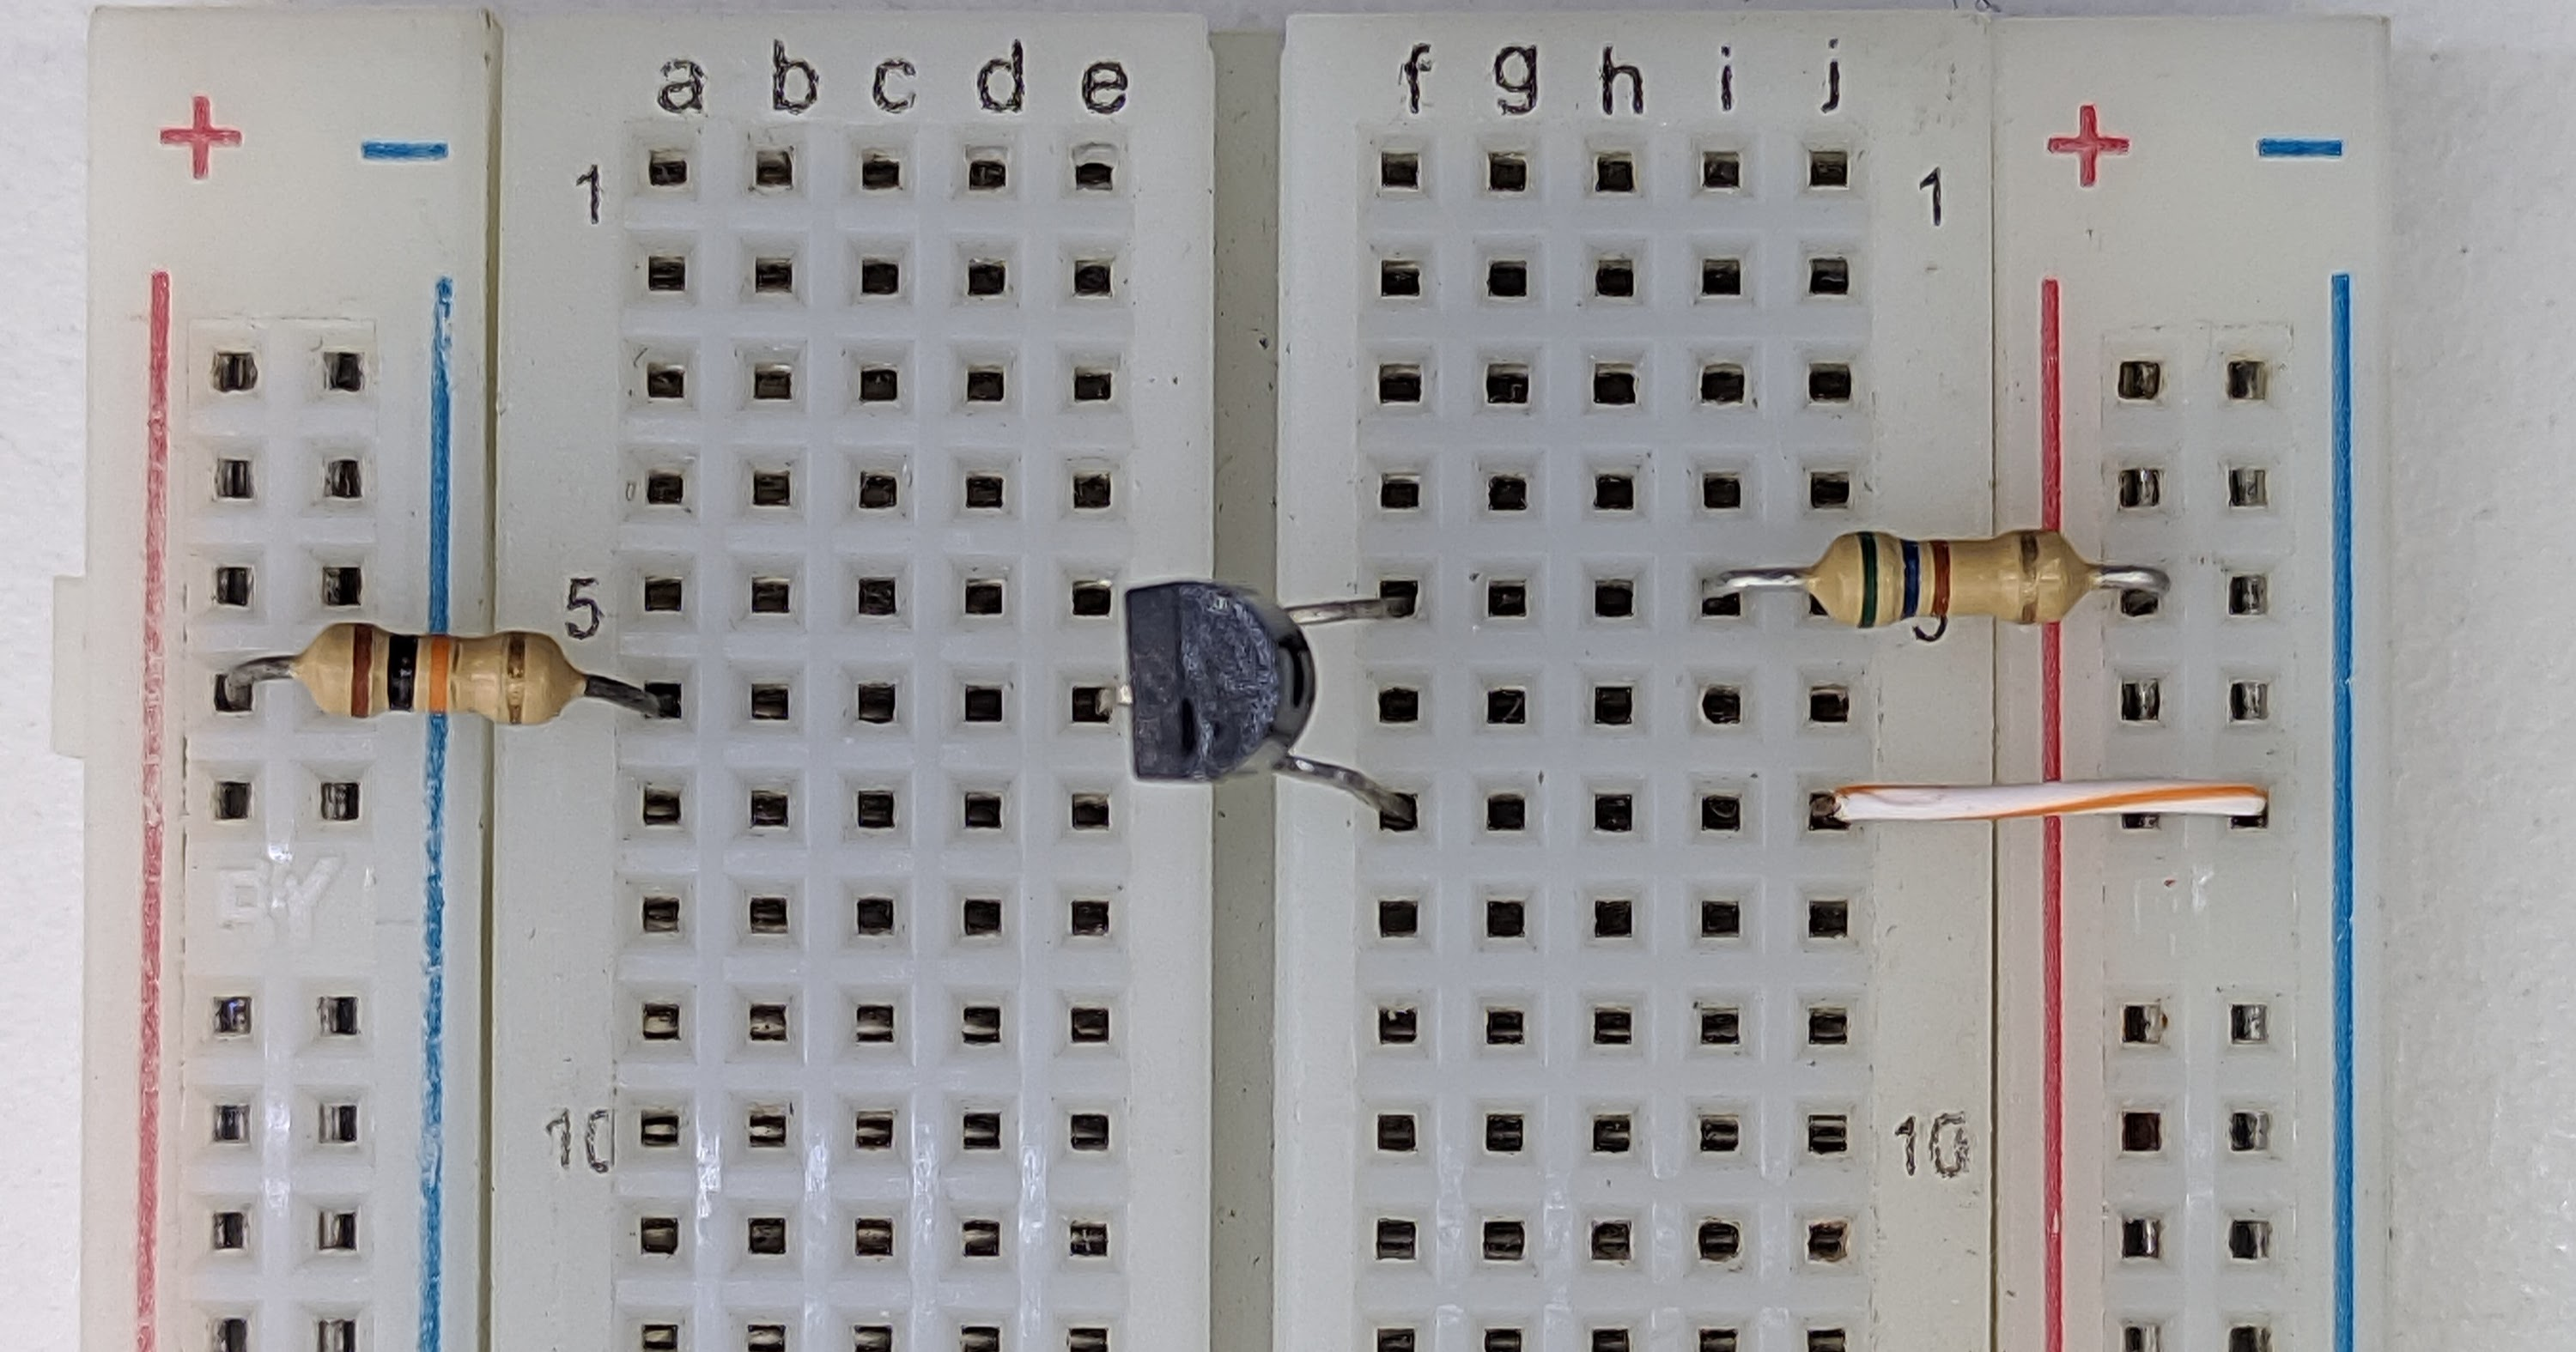
\includegraphics[width=0.3\textwidth]{pictures/prot_crkt-1.jpg}
      \caption{Circuito implementado.} 
      \label{fig:prot_polariz}
    \end{wrapfigure}
    Se pide realizar el mismo circuito implementado en la simulacion para poder ver su comportamiento cuando se polariza
    el transistor. En la figura (\ref{fig:prot_polariz}) se puede ver el circuito implementado en la protoboard.

    Una vez se tiene preparado el circuito se prosigue a prender la fuente y ver como actua el transistor mientra
    aumentamos el voltaje $V_{BB}$ para asi obtener los datos para completar la tabla.

    \begin{figure}[H]
      \centering
      \begin{minipage}{0.49\textwidth}
        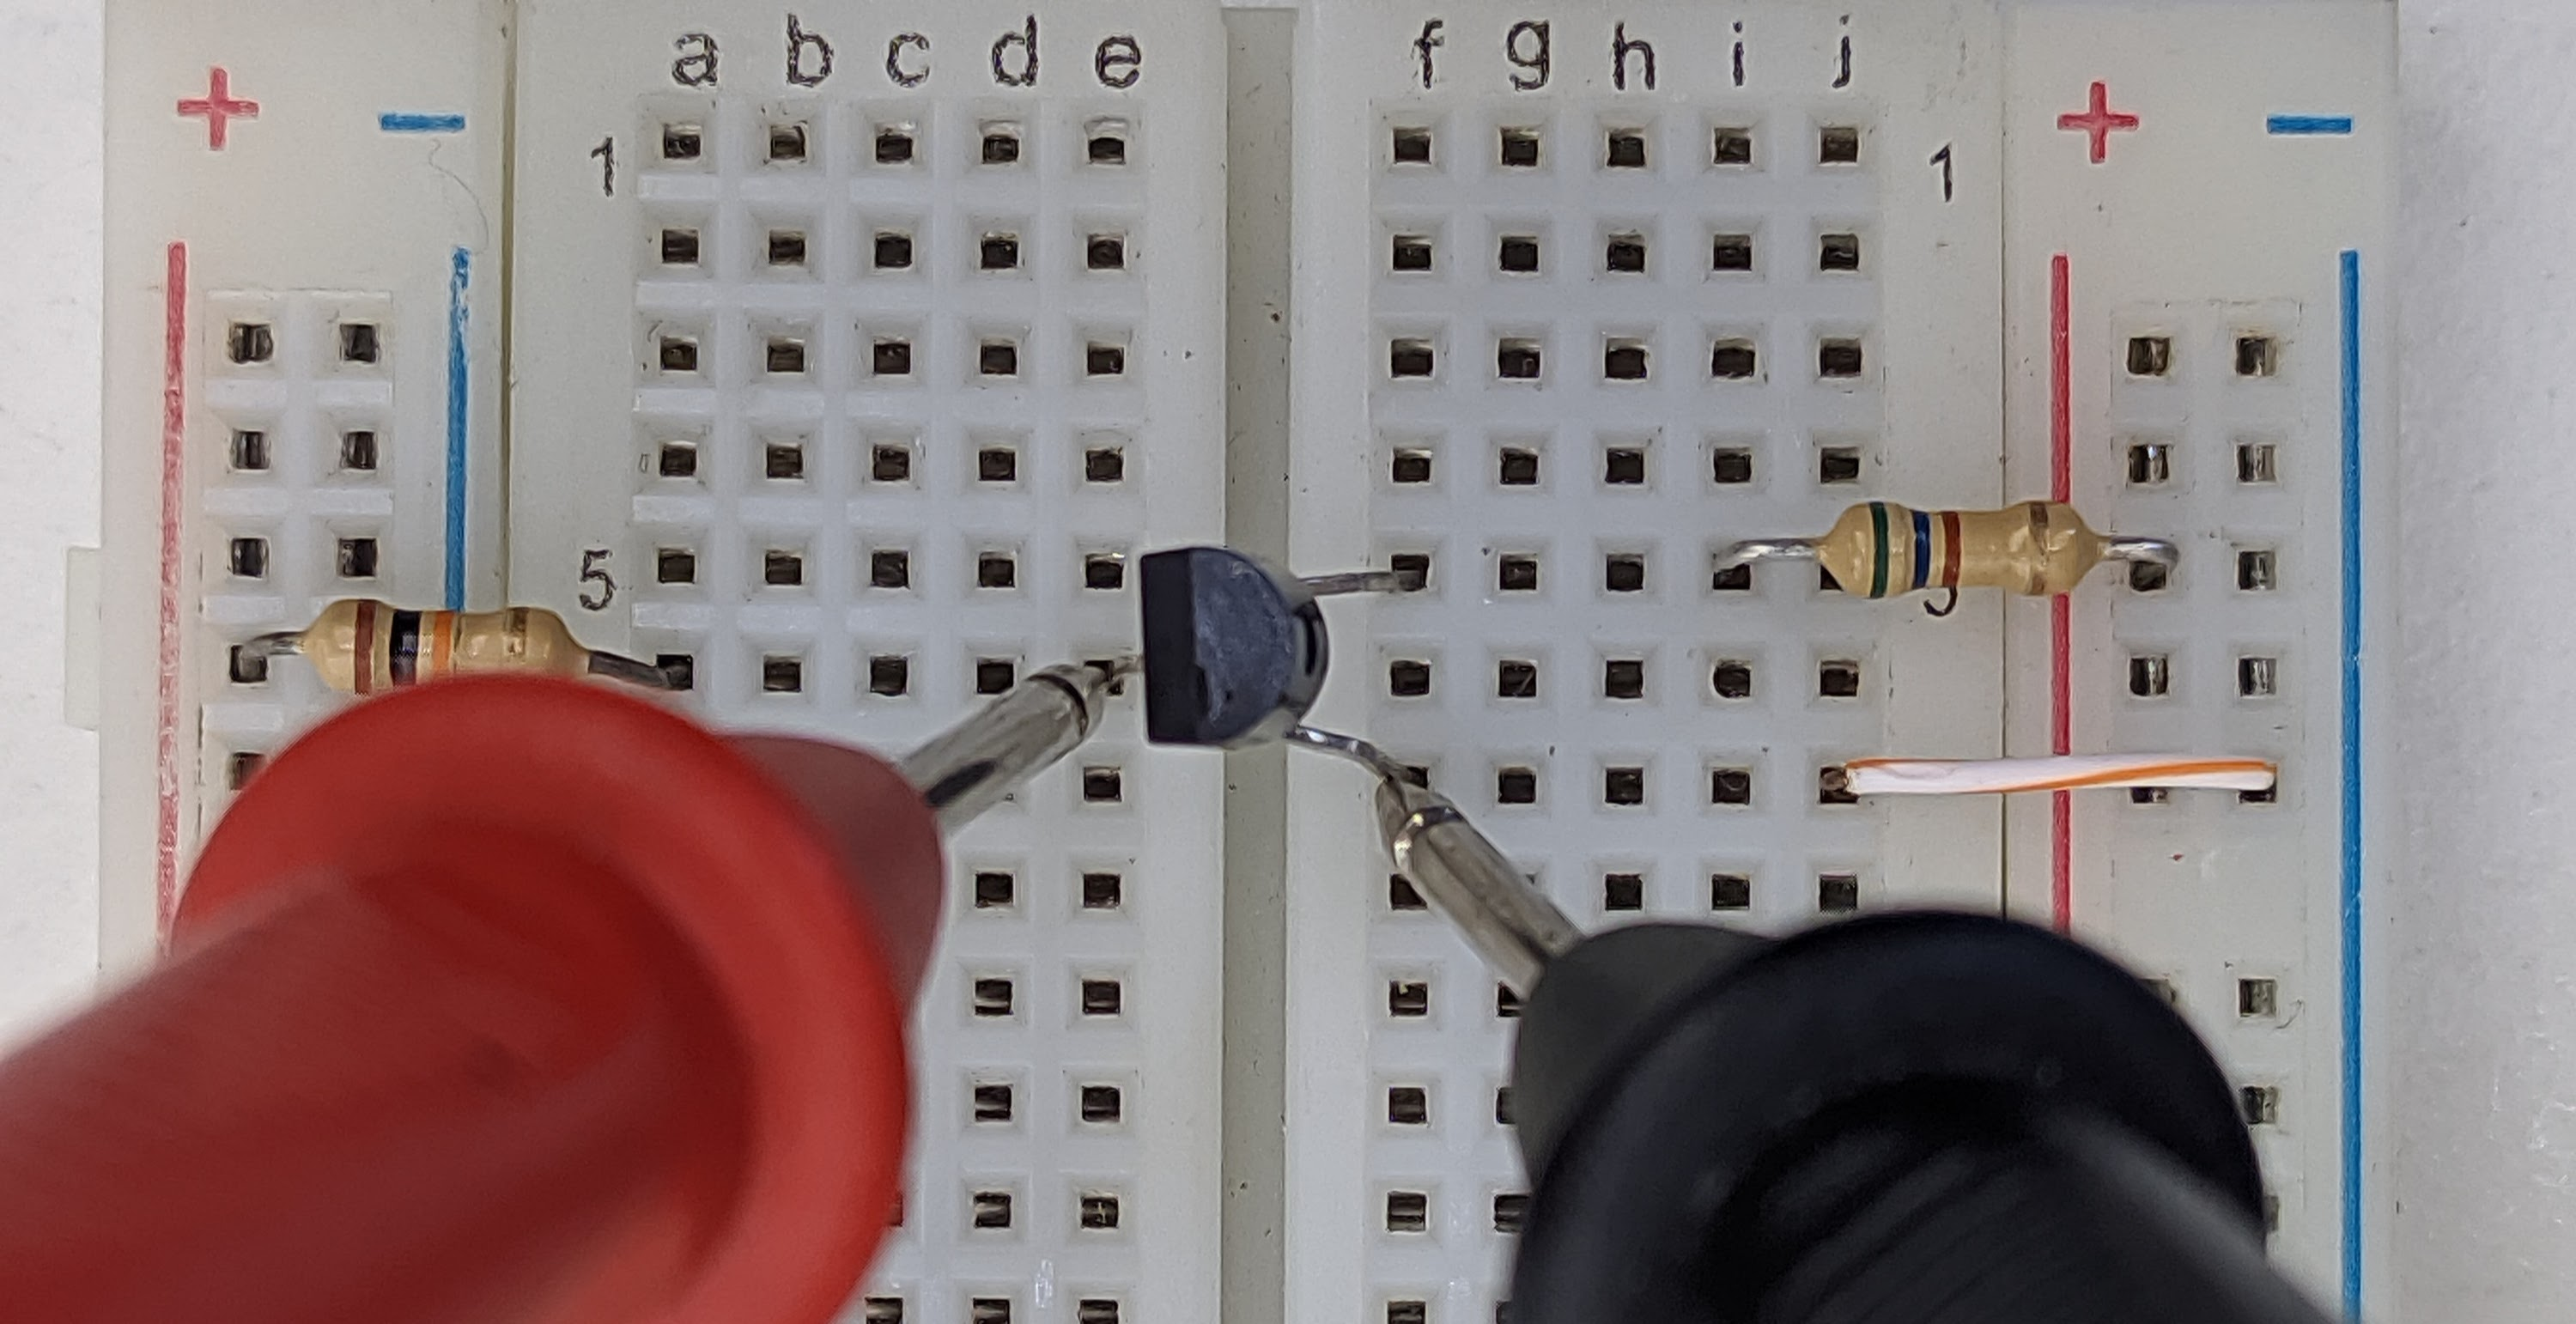
\includegraphics[width=1\textwidth]{pictures/prot_crkt-1_Vbe.jpg}
        \caption{Medicion de $V_{BE}$.}
      \end{minipage}
      \begin{minipage}{0.49\textwidth}
        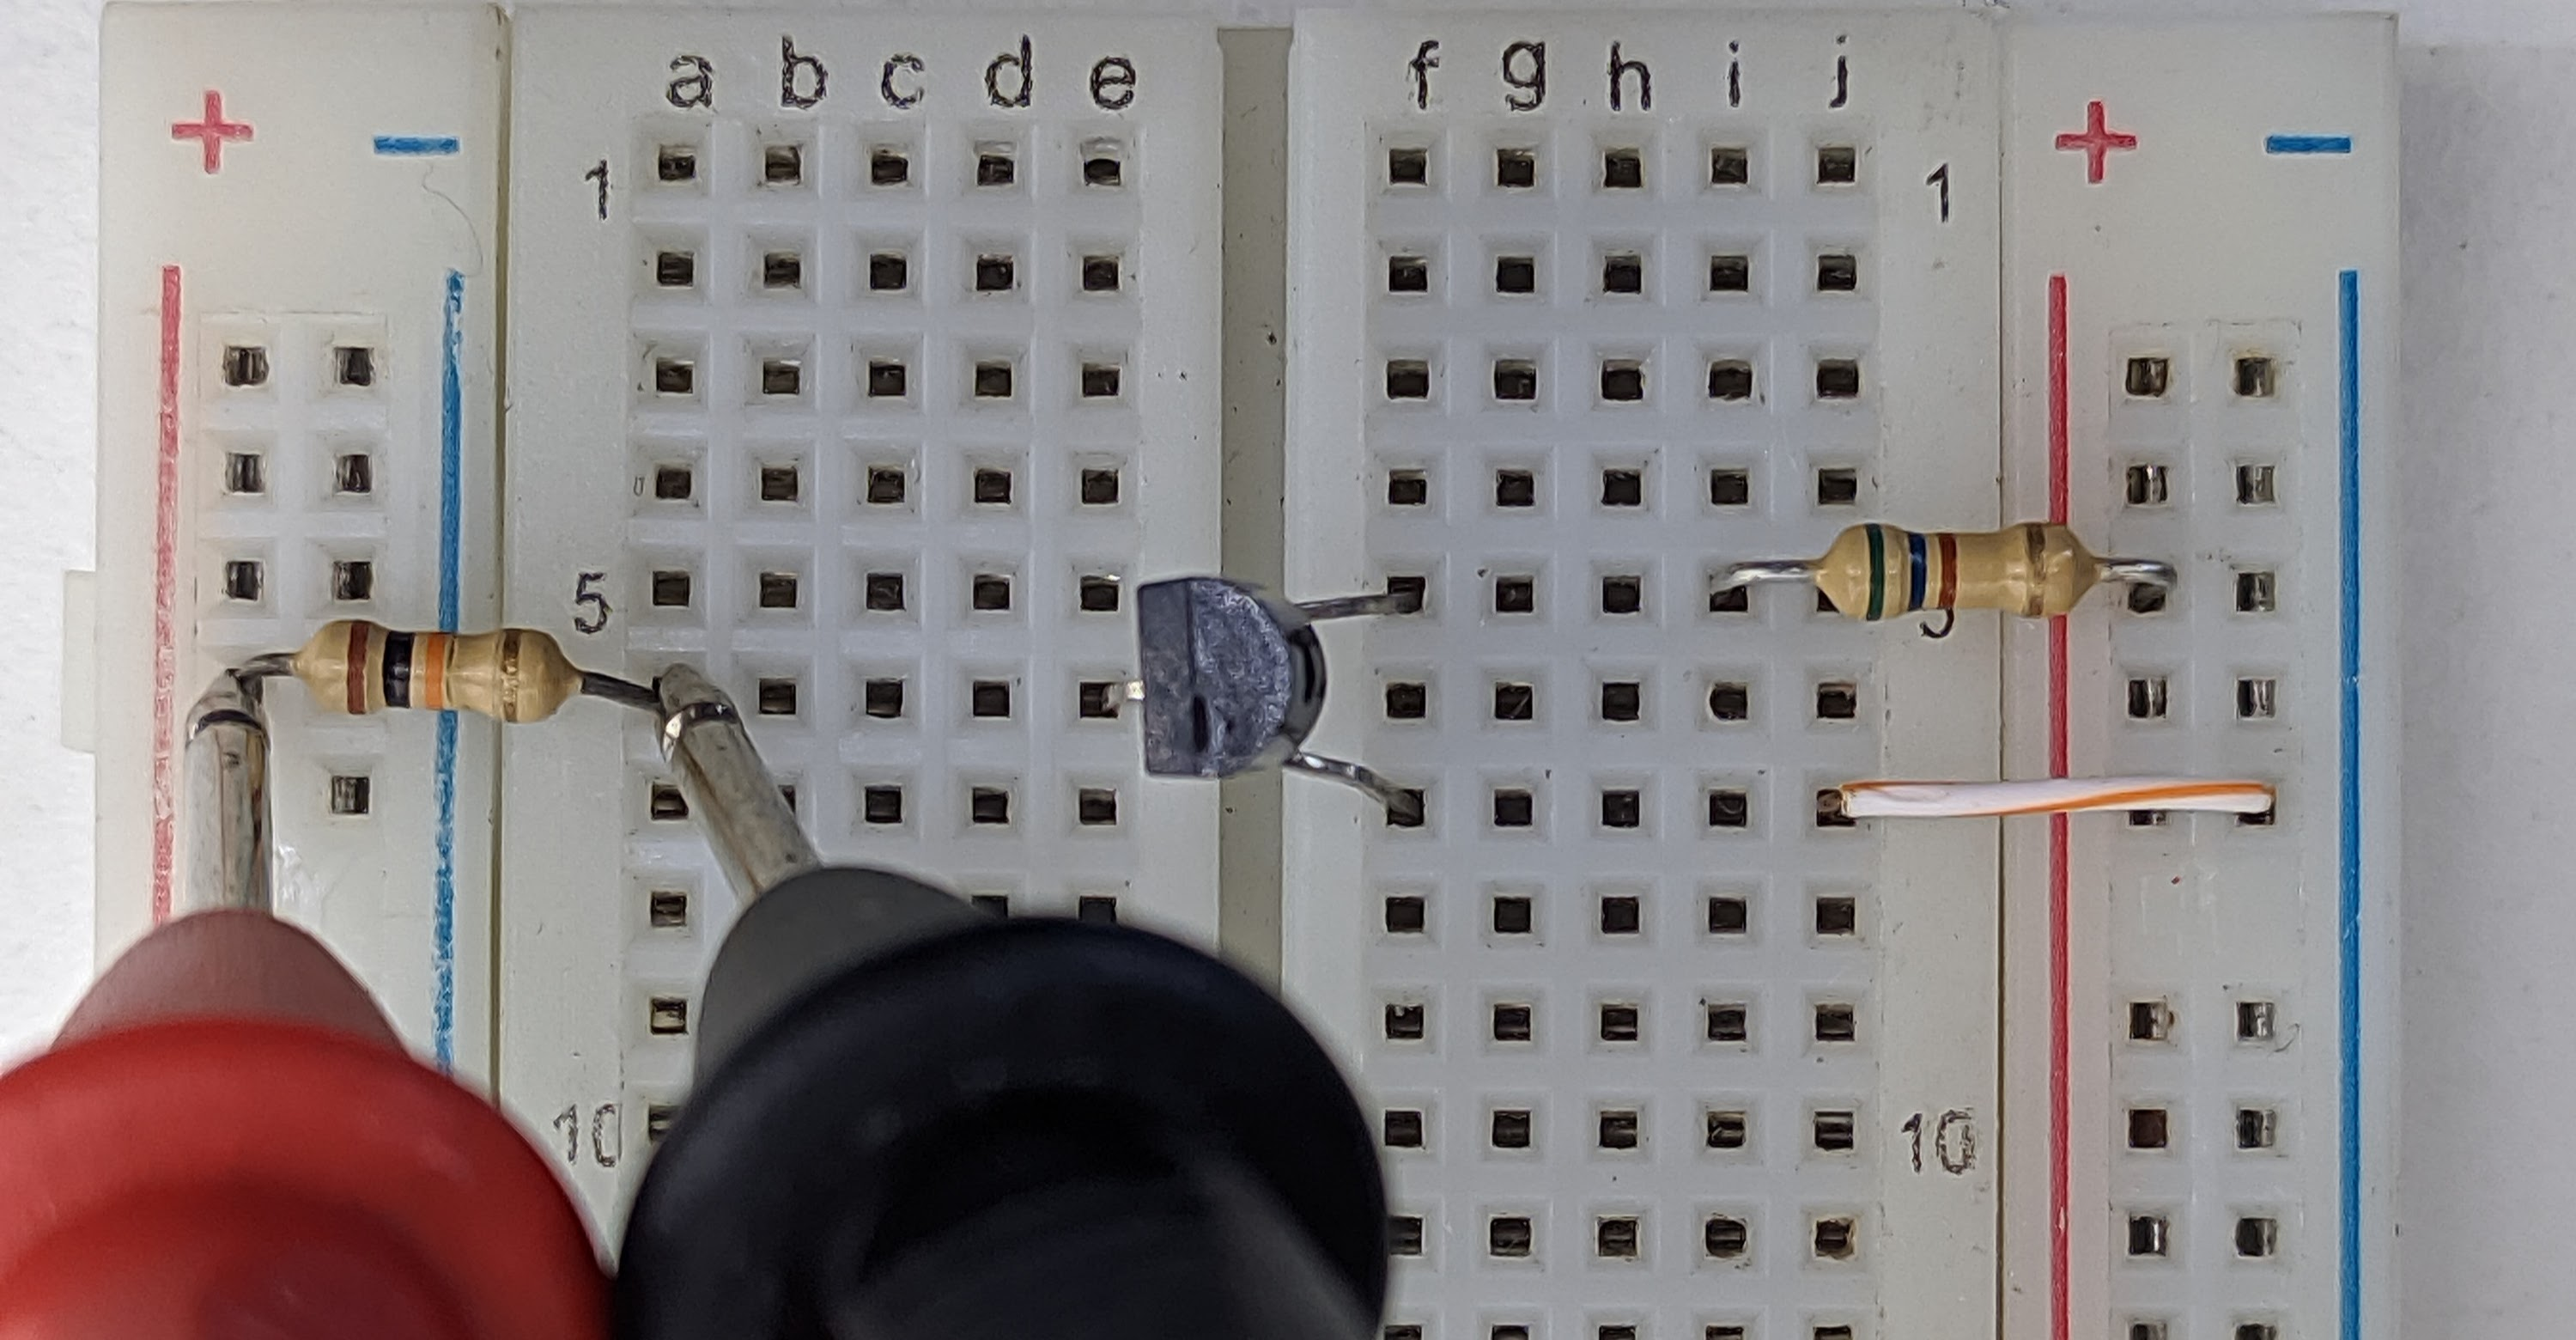
\includegraphics[width=1\textwidth]{pictures/prot_crkt-1_Vrb.jpg}
        \caption{Medicion de $V_{RB}$.}
      \end{minipage}
    \end{figure}

    Debido a que las corrientes de base son relativamente pequeñas para los multimetros comunes, decidimos que la
    medicion de la corriente se iba a hacer de manera indirecta. Para ello, los valores de corriente se obtienen de
    medir la caida de tension en la resistencia de base, dividirla por el valor de la resistencia, por lo que nos queda
    una ecuacion como como la siguiente:
    \begin{equation}
      I_B = \frac{V_{R_B}}{R_B}
    \end{equation}

    \begin{table}[h!]
      \centering
      \resizebox{\textwidth}{!}{
        \begin{tabular}{|c|c|c|c|c|c|c|c|c|c|c|c|}
          \hline
          $V_{BB}$   & $0\,V$ & $300\,mV$   & $400\,mV$   & $500\,mV$   & $600\,mV$ & $700\,mV    $ & $800\,mV      $ & $1\,V      $    & $3\,V        $  & $7\,V        $   & $10\,V       $ \\ \hline
          $I_B$      & $0\,A$ & $29\,nA $   & $40\,nA $   & $74\,nA $   & $739\,nA$ & $5.64\,\mu A$ & $18.34\, \mu A$ & $47\, \mu A$    & $225 \, \mu A$  & $625 \, \mu A$   & $742 \, \mu A$ \\ \hline
          $V_{BE}$   & $0\,V$ & $317\,mV$   & $395\,mV$   & $496\,mV$   & $591\,mV$ & $600\,mV    $ & $614\,mV      $ & $646\,mV   $    & $752\,mV     $  & $765\,mV     $   & $2.59\,V     $ \\ \hline
        \end{tabular}
      }
      \caption{Mediciones de $I_B$ y $V_{BE}$ para diferentes valores de $V_{BB}$.}
    \end{table}

    \begin{figure}[h!]
      \centering
      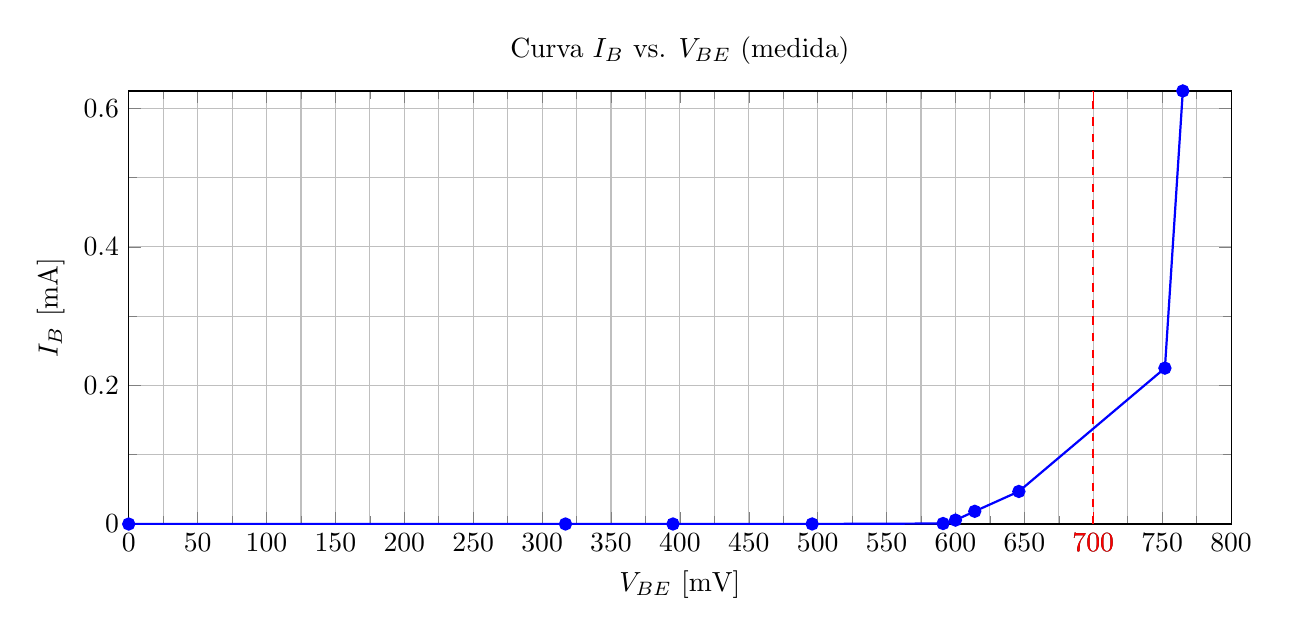
\begin{tikzpicture}
        \begin{axis}[
              width=14cm,
              height=5.5cm,
              xlabel={$V_{BE}$ [mV]},
              ylabel={$I_B$ [mA]},
              grid=both,
              minor tick num=1,
              scale only axis,
              enlargelimits=false,
                title={Curva $I_B$ vs. $V_{BE}$ (medida)},
              extra x ticks={700},
              extra x tick style={
                grid style={red, thick, dashed},
                tick style={red},
                tick label style={red}
               },
              scaled ticks=false,
              restrict x to domain=0:800,
              xmin=0, xmax=800
          ]
          \addplot[
              mark=*,
              color=blue,
              thick
          ] coordinates {
              (0, 0)
              (317, 29e-6)
              (395, 40e-6)
              (496, 74e-6)
              (591, 739e-6)
              (600, 5.64e-3)
              (614, 18.34e-3)
              (646, 47e-3)
              (752, 225e-3)
              (765, 625e-3)
          };
        \end{axis}
      \end{tikzpicture}
      \caption{Gráfico de la corriente de base $I_B$ en función de la tensión $V_{BE}$}
    \end{figure}

    \begin{wrapfigure}{l}{0.4\textwidth}
      \centering
      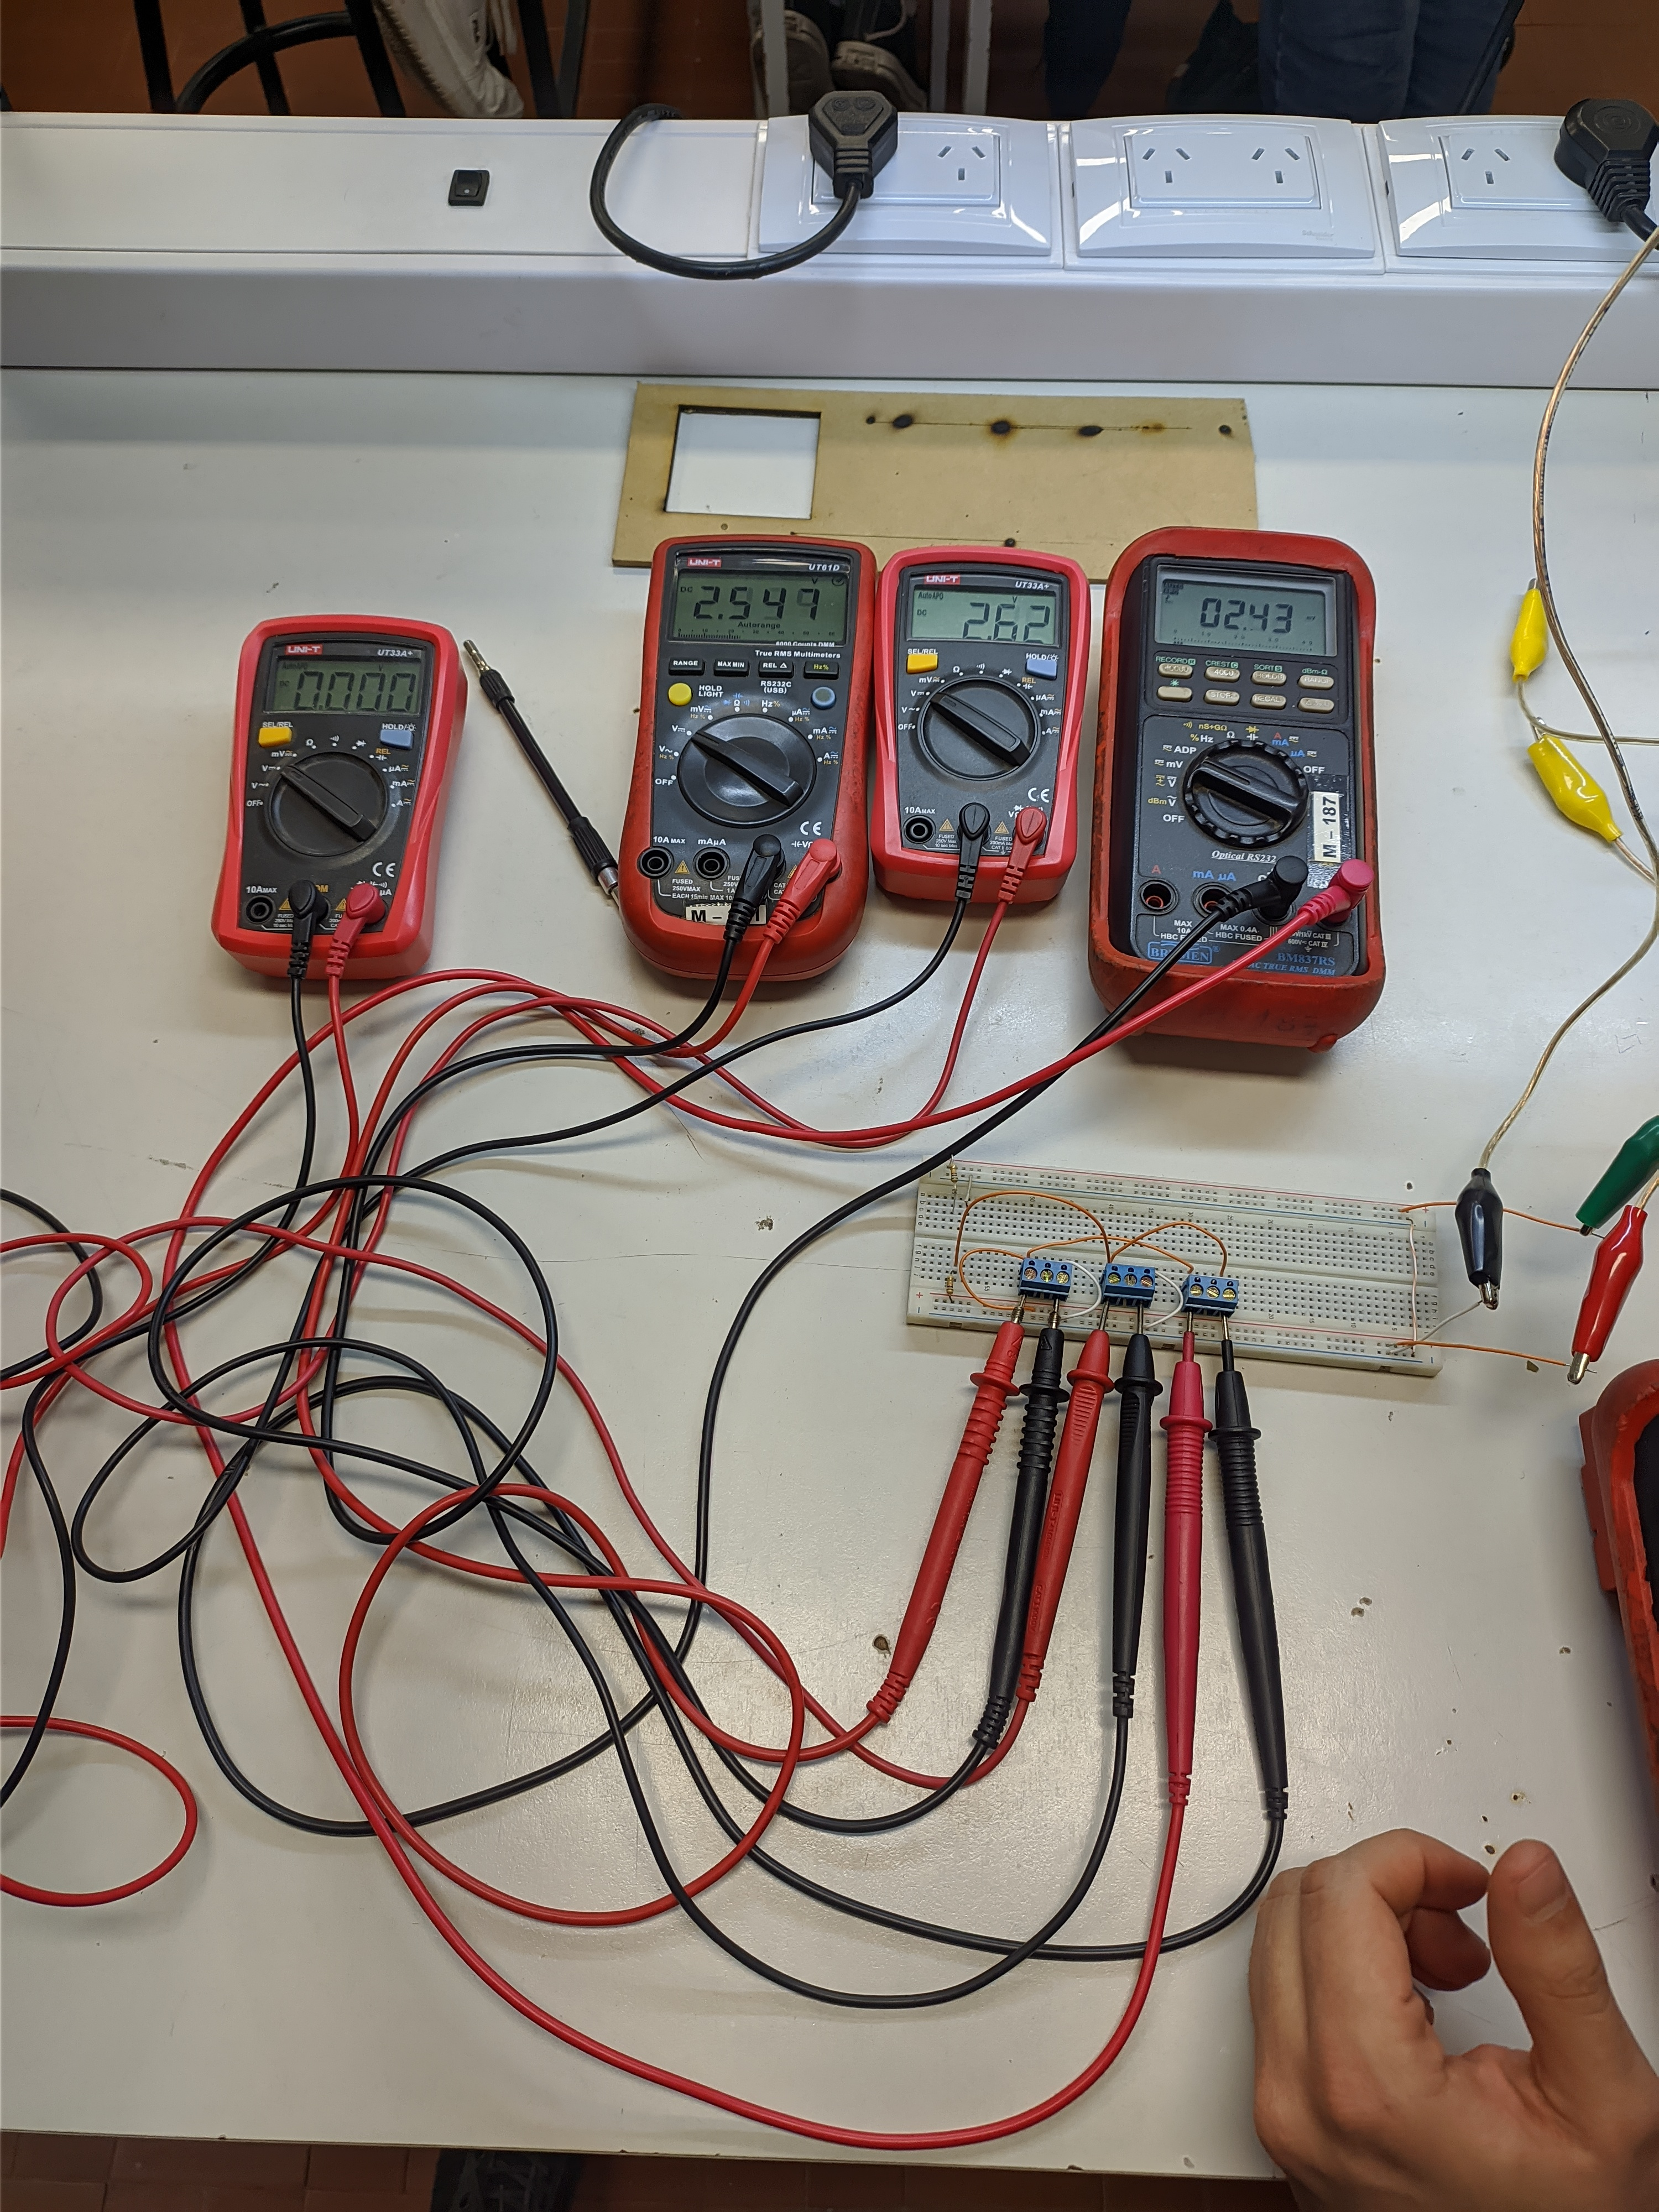
\includegraphics[width=0.35\textwidth]{pictures/setup_crkt-1.jpg}
      \caption{Circuito armado en el laboratorio.}
    \end{wrapfigure}
    A partir de mediciones experimentales, se observamos que la tensión $V_{BE}$ necesaria para que comience la
    conducción se encuentra en el rango típico de los diodos de silicio, aproximadamente entre $0.6\,V$ y $0.7\,V$.
    Ademas, las mediciones coinciden con el modelo simulado del transistor, lo que confirma que el control de corriente
    en el BJT está fuertemente determinado por la polarización de esta juntura.
